
\subsection{Compiler innovation: revisiting quantum programs} 

% To develop a highly effective en-to-end compiler, it is necessary to re 

% Different from 


Different from most existing sophisticated compilers tailored to $\CNOT$-based ISA, we reexamine the generic characteristics of quantum programs themselves beyond 1Q/2Q gate sequence representation to exploit the optimization opportunities that previous compiling strategies have overlooked. Real-world quantum algorithms can essentially be divided into two types: 1) those designed for solving classical problems and naturally represented as quantum versions of digital logic functions through binary encoding and 2) those for quantum or optimization problems typically constructed through Hamiltonian simulation. We name them \textit{Type-I --- digital-application programs} and \textit{Type-II --- simulation-application programs}, respectively. Detailed attributes of these two types of quantum programs are listed in \Cref{tab:programs}.


\begin{table}[tbp]
    \centering
    \caption{Quantum program categorization.}
    \label{tab:programs}
    \scalebox{0.95}{
    \begin{tabular}{|l||p{3cm}|p{3.2cm}|}
        \hline
        \textbf{Class} & \textit{Type-I} & \textit{Type-II} \\
        \hline
        \textbf{Usage} & Classical problems & Quantum / Optimization \\
        \hline
        \textbf{Construction} & Digital circuit components (data encoding similar to classical-world) & Hamiltonian simulation (Trotter decomposition) \\
        \hline
        \textbf{Execution} & Single-run to solve & Variational (Multiple-run)\\
        \hline
        \textbf{Examples} & ALU, Adder, Comparator, QFT, Grover & QAOA, VQE, UCCSD \\
        \hline
        \textbf{Program's IR} & $\mathrm{X}$/$\mathrm{CX}$/$\mathrm{CCX}$/$\mathrm{MCX}$; IR's arrangements are fixed & Pauli exponentiations; IR's arrangements are variable\\
        \hline
    \end{tabular}
    }
\end{table}



% These distinct program features offer valuable insights for designing program-adaptive compiling passes.

% Specifically, following are valuable insights we can leverage to design adaptive compiling strategies:
% \begin{itemize}
%     \item ...
%     \item ...
% \end{itemize}
% by inspecting program features:

Existing template-based~\cite{maslov2008quantum,bravyi2021clifford} and peephole~\cite{prasad2006data,sivarajah2020t} optimization techniques excel with $\CNOT$-based circuits for both Type-I and Type-II programs but overlook the program attributes thus the optimization space is severely limited, albeit some of them adopt high-level IR~\cite{li2022paulihedral,van2023towards}. Instead, ReQISC compiler takes program features (running mode, IR components, etc.) into account to tailor program-adaptive compiling passes for the $\SU(4)$ synthesis characteristics. Specifically, Type-I programs are composed of $\mathrm{X}$/$\mathrm{CX}$/$\mathrm{CCX}$/$\mathrm{MCX}$, sometimes with 1Q rotation gates. \Cref{fig:program_example} (a) shows examples of typical Type-I programs incorporating high-level semantics beyond 1Q/2Q gates. Therefore, it is reasonable to first find the optimal synthesis schemes for these finite IRs and then unroll them within quantum circuits. That is also due to the consideration of managing gate calibration overhead. Our compiler aligns this template-based optimization strategy by fixing 3Q as the grain of IR for synthesis. On the one hand, intricate circuit components such as Peres~\cite{thapliyal2009design}, MAJ, and UMA~\cite{cuccaro2004new} subroutines are usually represented as 3Q circuits. On the other hand, since we would like to attain the best template in $\SU(4)$ synthesis for some given IR, the approximate synthesis method is still required such that 3Q is the most proper granularity, while for multi-controlled-X ($\mathrm{MCX}$) gates, it can be recursively decomposed into $\mathrm{CCX}$s~\cite{barenco1995elementary}. Type-II programs are constructed from Hamiltonian simulation processes and executed in a variational manner. For instance, the 1D Heisenberg model depicted in \Cref{fig:program_example} (b), comprising neighboring $\mathrm{XX}$, $\mathrm{YY}$, $\mathrm{ZZ}$ interactions and local evolution terms, exemplifies this structure. To harness the disciplined global subprogram patterns inherent in Type-II programs, it is advisable to directly analyze their algorithmic expressions such as Hamiltonian models. Moreover, as variational quantum algorithms~\cite{cerezo2021variational}, Type-II programs necessitate multiple runs to update circuit parameters. Instead of continuously feeding a variational circuit to a conventional black-box compiler after each parameter update, a more efficient approach is to establish a circuit-structure-dependent but circuit-parameter-independent compiling scheme --- dubbed \dquote{structural compiling} in our study. By means of this scheme, circuit parameter updates are directly integrated into the compiled circuit without compiling once more. In ReQISC compiler, Pauli exponentiations (Pauli strings with coefficients) are regarded as native representations of Type-II programs such that the compilation problem is formulated as simplifying these unarranged Pauli exponentiations. By means of \dquote{binary symplectic form} (BSF)~\cite{van2020circuit} representation of Pauli strings and Clifford formalism, we proposed a heuristic algorithm \textit{BSF simplification} to simplify these Type-II programs' IRs.



\begin{figure}[tbp]
    \centering
    \subfigure[Type-I program example]{
        \includegraphics[width=0.43\columnwidth,trim={0.9cm 0 0 0},clip]{figures/type_I_example.png}
    }
    \subfigure[Type-II program example]{
        \includegraphics[width=0.5\columnwidth,trim={0 0 2cm 0},clip]{figures/type_II_example.png}
    }
    \caption{Examples of different categories of quantum programs. (a) \code{4mod7-v0\_94} and \code{ripple\_adder\_2} programs, which incorporate $\mathrm{CCX}$/$\mathrm{MCX}$ and $\mathrm{MAJ}$/$\mathrm{UMA}$ as high-level IRs. $\mathrm{MCX}$ are unrolled through schemes shown at the upper right of subfigure (a).  (b) 5-spin non-periodic 1D Heisenberg model composed of homogeneous near-neighbor $\mathrm{XX}$/$\mathrm{YY}$/$\mathrm{ZZ}$ couplings and individual $Z$-axis spin Hamiltonians. The Trotterized circuit comprises a sequence of Ising gates and $R_z$ gates with different rotation angles.}
    \label{fig:program_example}
\end{figure}







% Type-I programs exhibit versatile fine-grained subcircuit


% \begin{itemize}
%     \item Type-I programs ... \ZY{(key attributes \& examples)}
%     \item Type-II programs ... \ZY{(key attributes \& examples)}
% \end{itemize}

\begin{figure}[tbp]
    \centering
    \subfigure[Type-I program compiling]{
        % \includegraphics[width=0.56\columnwidth,trim={2.1cm 0 0 0},clip]{figures/type_I_pass.png}
        \includegraphics[width=0.55\columnwidth]{figures/type_I_pass.png}
    }
    \subfigure[Type-II program compiling]{
        % \includegraphics[width=0.37\columnwidth,trim={2.2cm 0 0 0},clip]{figures/type_II_pass.png}
        \includegraphics[width=0.38\columnwidth]{figures/type_II_pass.png}
    }
    \caption{Program-adaptive synthesis. (a) For Type-I programs, input $\mathrm{CCX}$-based circuits are partitioned into refined 3Q IRs, which are subsequently assembled by searching the optimal schemes from a pre-synthesized template library across a benchmark suite. (b) For Type-II programs, input Pauli exponentiations are grouped and then passed through BSF simplification procedure for each group. Finally, simplified BSFs and Clifford2Q conjugations are organized into 1Q/2Q gate sequences and rebased to $\SU(4)$ circuits.}
    \label{fig:program_adaptive}
\end{figure}






\textbf{BSF simplification for Type-II program:} Conventionally, Type-II programs are constructed through Trotterizing~\cite{dalzell2023quantum} the unitary evolution operator under a given Hamiltonian. An arbitrary Hamiltonian can be expressed as a linear combination of Pauli strings
\begin{align}
    H = \sum_{j=1}^L h_j P_j = \sum_{j=1}^L h_j \sigma_0^{(j)} \otimes \cdots \otimes \sigma_{n-1}^{(j)}.
\end{align}
To represent unitary evolution $U(t) = e^{-iHt}$ under $H$ into quantum circuits, it is usually approximately decomposed into multi-step evolutions --- Trotterization, each of which is the product of individual Pauli exponentiations during a little time slice. Then the product of Pauli exponentiations could be trivially converted to 1Q/2Q circuits. The Trotterization theory is under the assumption that the product of matrix exponentiations is a good approximation for the sum of matrix exponentiations. Specifically, 
\begin{align}
    U(t) = e^{-iHt} \simeq  \left( S_{k}\left(\tau\right) \right)^r,\, \tau = \frac{t}{r}
\end{align}
is called $r$-step Trotterization, in which the $k$-th order inner product formula $S_k(\tau)$ is in the following forms:
\begin{align*}
    &S_1 = \prod_{j=1}^{L} \exp^{ -i h_j \tau P_j},\,
    S_2 = \prod_{j=1}^{L} \exp^{ -i h_j \frac{\tau}{2} P_j}\prod_{j=L}^1 \exp^{ -i h_j \frac{\tau}{2} P_j},\\
    &S_{2k}(\tau) = [S_{2k-2}(p_k\tau)]^2S_{2k-2}\left( (1-4p_k)\tau\right)[S_{2k-2}(p_k\tau)]^2,
\end{align*}
where $p_k = 1 / ( 4 - 4^\frac{1}{2k-1})$ and $k > 1$. After Troterrization, each Pauli exponentiation can be exactly synthesized by $\CNOT$s and 1Q rotations. The Trotter approximation errors result from non-commuting terms in the Hamiltonian since $ e^{A+B} = e^{A} e^{B} = e^{B} e^{A} $ is satisfied only when $[A,B]=0$. However, in practice, according to the analysis of theoretical Troterization error~\cite{dalzell2023quantum} and our field-test results of different arrangements Pauli exponentiations (e.g., 1-order Trotterization error $\mathcal{O} ( \lVert H\rVert_1^2 \, t^2 / r )$, 2-order Trotterization error $\mathcal{O} ( \lVert H\rVert_1^3 \, t^3 / r^2 )$)\footnote{Our field work suggests the infidelity is in the order of magnitude $10^{-4}$ in 1-order 1-step Trotterization, $10^{-5}$ in 1-order 2-step Trotterization and $10^{-7}$ in 2-order 2-step Trotterization under a normalized Hamiltonian (coefficients in Pauli exponentiation could be in the order of magnitude $10^{-3}$-$10^{-2}$). Neither the order of Pauli strings (or grouping scheme) nor the number of qubits matters significantly in approximation error and infidelity. This error is small enough for us to be confident that the rearranged Trotterized circuit is also a good ansatz for variational algorithms.}, the compilation error resulting from rearranging Trotterized Pauli exponentiations is negligible. On the other hand, for variational execution, we can take the rearranged Pauli exponentiations as the new Trotterized circuit as the ansatz, thereby eliminating the effects of any compilation errors. A good analogy to this insight could be the prevalent \dquote{pruning + fine-tuning} approach to compressing neural networks in the area of machine learning systems, which is capable of substantially reducing NN's weights while preserving or even improving NN's prediction accuracy. In this sense, it is reasonable to invent a global Pauli exponentiation scheduling approach for exhaustively optimizing Type-II programs.


\begin{figure}[tbp]
    \centering
    % \subfigure[Trivial approach to synthesizing Pauli exponentiations]{
        \input{circuits/xxx_xyy}
    % }
    \vspace{0.2cm}
    % \subfigure[Simplified Pauli exponentiations by Clifford2Q]{
        \input{circuits/xxx_xyy_simplified}
    % }
    \caption{Pauli exponentiation synthesis v.s. simplification by Clifford2Q. We use Pauli equivalence rules $X(\theta) = H\, Z(\theta)\, H$ and $Y(\theta) = SHS\, Z(\theta)\, S^\dagger H S^\dagger = \mathrm{U}3(-\frac{\pi}{2},-\frac{\pi}{2},\frac{\pi}{2})\, Z(\theta)\, \mathrm{U}3(\frac{\pi}{2}, -\frac{\pi}{2}, \frac{\pi}{2})$. }
    \label{fig:xxx-xyy-simp}
\end{figure}

The example in \Cref{fig:xxx-xyy-simp} gives a taste of the synthesis approach for Type-II programs. Pauli exponentiations $ e^{-i (\frac{\phi}{2}XYY + \frac{\theta}{2}XXX)} $ necessitate two V-shaped $\CNOT$ trees, resulting in 6 2Q gates. However, If the circuit is conjugated by the Clifford transformation $ \CNOT_{1,0} $, it is simplified into two consecutive Ising gates acting on $(q_1, q_2)$, which can be synthesized by an $ \SU(4) $. This case implies that the significant improvement of synthesis effect for Pauli exponentiations can be achieved by applying appropriate Clifford transformations.


To formulate our synthesis scheme, % in a unified perspective, 
we represent Pauli strings in \textit{binary symplectic form} (BSF)~\cite{van2020circuit}. BSF is a tableau representation in which each row represents a single $ n $-qubit Pauli string. Columns of the tableau are partitioned as two parts $ [X\,|\,Z] $, such that $ [X_{i,j}\,|\, Z_{i,j}] $ represents the $ j $-th component of the $ i $-th Pauli operator. The value is $ [1 | 0 ] $ for $ X $, $ [0 | 1 ] $ for $ Z $, $ [1 | 1 ] $ for $ Y $, and $ [0 | 0 ] $ for $ I $. For instance, the process in\Cref{fig:xxx-xyy-simp} that Pauli strings $ [XXX; XYY] $ is transformed into $ [IXX; IYY] $ is formulated as 
\begin{align*}
    \left[
        \begin{array}{ccc|ccc}
        1 & 1 & 1 & 0 & 0 & 0 \\
        1 & 1 & 1 & 0 & 1 & 1
        \end{array}
    \right]
    \xrightarrow{C(Z,X)_{1,0}}
    \left[
        \begin{array}{ccc|ccc}
            0 & 1 & 1 & 0 & 0 & 0 \\
            0 & 1 & 1 & 0 & 1 & 1
        \end{array}
    \right].
\end{align*}
To characterize the general Clifford transformation effects on BSF, we use the \textit{universal controlled gate} 
\begin{align}
    C(\sigma_0, \sigma_1) = \frac{1}{2}((I + \sigma_0)\otimes I + (I - \sigma_0)\otimes \sigma_1)
\end{align}
where $ \sigma_0,\sigma_1\in \left\{X,Y,Z\right\} $. For example, $C(Z,X)$ is $\CNOT$.

% \begin{figure}[tbp]
%     \centering
%     \subfigure[$H$ transformation]{
%         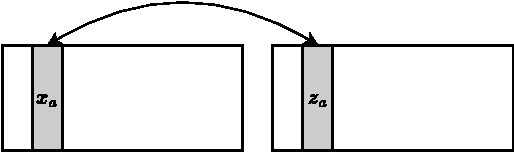
\includegraphics[width=0.45\columnwidth]{figures/H.pdf}
%     }\quad
%     \subfigure[$S$ transformation]{
%         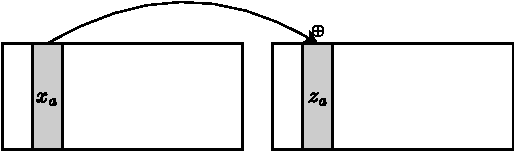
\includegraphics[width=0.45\columnwidth]{figures/S.pdf}
%     }\\
%     \subfigure[$C(Z,X)$ transformation]{
%         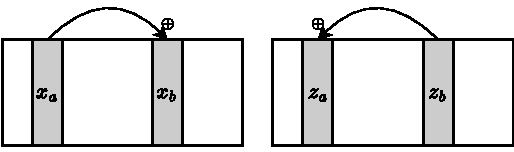
\includegraphics[width=0.45\columnwidth]{figures/C(Z,X).pdf}
%     }\quad
%     \subfigure[$C(X,X)$ transformation]{
%         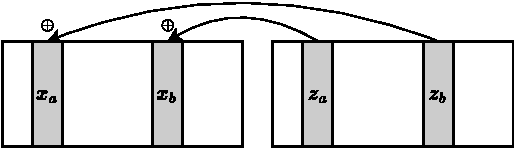
\includegraphics[width=0.45\columnwidth]{figures/C(X,X).pdf}
%     }
%     \caption{Examples of Clifford transformation on the BSF representation of Pauli strings. Columns $a$ and $b$, corresponding to qubit $a$ and $b$, for $X$ and $Z$ blocks are indicated by $x_a$, $x_b$, $z_a$, $z_b$, respectively. (a) $H$ gate acting on qubit $a$ will exchanges $x_a$ and $z_a$. (b) $S$ gate acting on qubit $a$ results in $z_a \gets z_a \oplus x_a$. (c) $C(Z,X)_{a,b}$, i.e., the $\CNOT$ gate, results in $x_b \gets x_b \oplus x_a$ and $z_a \gets z_a \oplus z_b$. (d) $C(X,X)$ transformation is equivalent with successively applying $H$ on $a$, $C(Z,X)_{a,b}$, and $H$ on $a$, which leads to $x_a \gets x_a \oplus z_b$ and $x_b \gets x_b \oplus z_a$.}
%     \label{fig:cliff-trans-on-bsf}
% \end{figure}


In general, a set of Pauli strings can be synthesized by an $\SU(4)$ if and only if the intersection of weights from every Pauli string lies in at most two qubits. In other words, the so-defined \dquote{$\totalWeight$}
\begin{align}
    \lVert  \lor_i (r_x^{(i)}\lor r_z^{(i)})  \rVert \leq 2,
    \label{eq:bsf_simplest}
\end{align}
where $r_{x/z}$ is the $r$-th row of $X$ or $Z$ block of the BSF, and the norm is the sum of all binary entries. The example in \Cref{fig:xxx-xyy-simp} shows how $\CNOT_{1,0}$ conjugation simultaneously simplifies $XXX(\theta)$ and $XYY(\theta)$ into Pauli strings only acting on $(q_1, q_2)$. To generalize this procedure, we need to make explicit the formalism of how Cliffords transform the Pauli group.

Operators $C$ from the Clifford group are unitary and have the property that $CPC^\dagger$ is also a Pauli operator for any Pauli operator $P$. % The Clifford group can be generated by three basic gates $\left\{H,S,\CNOT\right\}$.
Only 2Q Clifford operators (Clifford2Q) potentially have non-trivial effects on simplifying tableau weights of BSF aimed at straightforward $\SU(4)$ synthesis, as revealed through examining how the update rules of Clifford operators relate to the BSF~\cite{van2020circuit}.
% The update rules of some Clifford operators in terms of the BSF are shown in~\Cref{fig:cliff-trans-on-bsf}, in which only Clifford2Q operators potentially have non-trivial effects on simplifying tableau weights targeted for straightforward $\SU(4)$ synthesis. 
To search suitable Clifford2Q operators, it suffices to just focus on a set of 2Q generators of the 2Q Clifford group. In Clifford group theory, the 6 universal controlled gates 
\begin{align*}
    \left\{ C(X,X), C(Y,Y), C(Z,Z), C(X,Y), C(Y,Z), C(Z,X) \right\}
\end{align*}
are independent of each other and span the entire 2Q Clifford group~\cite{grier2022classification}. Each of them can reduce the weight of certain Pauli strings. For example, $C(X,Y)\, [0\, 0\, |\, 1\, 1] \,C(X,Y) = [0\, 0\, |\, 1\, 0] $ since $C(X,Y)_{a,b}$ exhibits the rule
\begin{align*}
[x_a,\, x_b\, |\, z_a,\, z_b] \rightarrow [x_a\oplus x_b\oplus z_b,\, z_a\oplus z_b\, |\, z_a,\, z_a\oplus z_b].
\end{align*}
% Note all generators above are Hermitian and therefore are involutions. 

\begin{algorithm}[tbp]
    \SetAlgoLined
    \caption{Pauli Strings Simplification in BSF}
    \label{algo:simplification}
    \SetKwInOut{Input}{Input}
    \SetKwInOut{Output}{Output}
    \SetKwBlock{Assumption}{Assumption}{}

    % \Input{Pauli strings with corresponding coefficients (\textit{pls}, \textit{coes})}
    \Input{Pauli strings list \textit{pls}}
    \Output{Reconfigured circuit components list \textit{cfg}}

    % \tcp{Following pseudocode only involves transformation on pls while omitting coes WLOG}
    \BlankLine
    \textit{cfg} $ \gets \emptyset $;\quad
    \textit{bsf} $ \gets \textsc{BSF}$(\textit{pls});\quad
    \textit{cliffs\_with\_locals} $\gets \emptyset$\; %\tcp*{Cliffords with local Paulis}
    % $ n \gets $ \textit{bsf}.\textsc{numQubits}()\;
    \While{bsf.\textsc{totalWeight()} $>$ 2}{
        \textit{local\_bsf} $\gets$ \textit{bsf}.\textsc{popLocalPaulis}()\; 
        % $ C \gets \emptyset$;\quad
        % $ B \gets \emptyset$;\quad

        $ C \gets \emptyset$ \tcp*{Clifford2Q candidates}
        $ B \gets \emptyset$ \tcp*{Each element of $B$ results from applying each Clifford2Q candidate on \textit{bsf}}
        \textit{costs} $\gets \emptyset$ \tcp*{Cost functions calculated on each element of $B$}
        \For{cg \textbf{in} \textsc{CLIFFORD\_2Q\_SET}}{
            \For{i, j \textbf{in} $ \textsc{combinations}(\textsc{range}(n), 2) $}{
                \textit{cliff} $\gets$ \textit{cg}.\textsc{on}$ (i, j) $ \tcp*{qubits acted on}
                \textit{bsf}$'$ $\gets$ \textit{bsf}.\textsc{applyClifford2Q}(\textit{cliff})\;
                \textit{cost} $\gets$ \textsc{calculateBSFCost}(\textit{bsf}$'$)\;
                $ C.\textsc{append}$(\textit{cliff})\;
                $ B.\textsc{append}$(\textit{bsf}$'$)\;
                \textit{costs}.\textsc{append}(\textit{cost})\;
            }
        }
        % \textit{bsf} $\gets$ \textit{B}[\textit{costs}.\textsc{index}(\textit{min}(\textit{costs}))]\;
        % \textit{cliff} $\gets$ \textit{C}[\textit{costs}.\textsc{index}(\textit{min}(\textit{costs}))]\;
        \textit{bsf} $ \gets \textsc{BSFWithMinCost} (B, \textit{costs}) $\;
        \textit{cliff} $ \gets \textsc{CliffordWithMinCost} (C, \textit{costs}) $\;
        \textit{cliffs\_with\_locals}.\textsc{append}((\textit{cliff}, \textit{local\_bsf}))\;
    }
    \BlankLine
    \textit{cfg}.\textsc{append}(\textit{bsf})\;
    \For{cliff, local\_bsf \textbf{in} cliffs\_with\_locals}{
        \tcp{Clifford2Q operators are added as conjugations, with local Pauli strings peeled before each epoch}
        \textit{cfg}.\textsc{prepend}(\textit{cliff})\;
        \textit{cfg}.\textsc{append}(\textit{local\_bsf})\;
        \textit{cfg}.\textsc{append}(\textit{cliff})\;
    }

\end{algorithm}


To exploit such opportunities of simultaneously simplifying Pauli strings by conjugation of appropriate Clifford2Q operators, we present a heuristic algorithm to search for as few appropriate Clifford2Q generators as possible. \Cref{algo:simplification} illustrated the detailed procedure. Input is a set of Pauli strings and output is an $\SU(4)$-synthesizable Pauli string list with generators and local Pauli strings generated in each search epoch. %Since it is trivial to track corresponding coefficients when transforming Pauli strings, \Cref{algo:simplification} only involves Pauli strings \textit{pls}. 
The output represents a configuration list \textit{cfg}, in which each component is either a generator or a BSF with $\totalWeight$ defined in \Cref{eq:bsf_simplest} no more than 2. Either can be trivially converted into an executable subcircuit in the $\CNOT$-based or $\SU(4)$-based ISA. Local Pauli strings mean the weight of each is at most 1, which can be generated in intermediate Clifford transformation. Before each 
Clifford2Q search epoch, local Pauli strings are peeled from the BSF, because they represent 1Q gates and do not introduce $\SU(4)$ synthesis overhead. A detailed explanation of key steps is listed as follows:
\begin{itemize}
    % \item This algorithm is suitable for simplifying Pauli exponentiation although the input only includes Pauli strings \textit{pls} without coefficients, 
    \item The heuristic searching algorithm will first check if \textit{bsf}'s $\totalWeight$ is larger than 2, otherwise it searches a Clifford2Q generator that simplifies \textit{bsf} the most in each iterative epoch, until $\totalWeight \leq 2$. When calculating $\totalWeight$, local Pauli strings within \textit{bsf} are excluded. If $\totalWeight > 2$, the local Pauli strings are peeled from \textit{bsf} and are added into a different BSF tableau \textit{local\_bsf} and heuristic searching is performed on the updated \textit{bsf}. Otherwise, \textit{bsf} and \textit{cliffs\_with\_locals} are assembled into the output \textit{cfg}.
    % \item ... global coefficients (S\^dagger
    \item To determine which Clifford2Q to select, all Clifford2Q generators $\{C(\sigma_0, \sigma_1)\}$ with all possible qubit pairs in action are presumptively applied and ultimately the one that transforms \textit{bsf} into a BSF with the minimum cost function will be selected. Specifically, the cost function is defined as
    % \begin{align*}
    %     \sum_{\langle i,j \rangle}& \lVert r_x^{(i)} \lor r_z^{(i)} \lor r_x^{(j)} \lor r_z^{(j)} \rVert \, +\\ &\frac{1}{2} \sum_{\langle i,j \rangle} (\lVert r_x^{(i)} \lor r_x^{(j)} \rVert + \lVert r_z^{(i)} \lor r_z^{(j)} \rVert),
    % \end{align*}
    \begin{align*}
        \textrm{cost} =  n_\textrm{non\_trivial}^2 &* \left(\vphantom{\sum}\right. \sum_{\langle i,j \rangle} \lVert r_x^{(i)} \lor r_z^{(i)} \lor r_x^{(j)} \lor r_z^{(j)} \rVert  \\
        & + \frac{1}{2} \sum_{\langle i,j \rangle} (\lVert r_x^{(i)} \lor r_x^{(j)} \rVert + \lVert r_z^{(i)} \lor r_z^{(j)} \rVert)\left.\vphantom{\sum}\right)
    \end{align*}
    which is the combined weight overlap of both $X$-part and $Z$-part among each pair of Pauli strings in \textit{bsf}. This measures how far the current BSF is from being $\SU(4)$-synthesizable.
    %It is a reasonable cost function as the optimization proceeds, \textit{bsf}'s cost function gets lowered. 
    Of course all local Pauli strings are excluded when calculating this cost function. 
    % \item In the final stage of assembling intermediate results into \textit{cfg}, it first adds simplified \textit{bsf} into it. Then the searched Clifford2Q operators as conjugations are added subsequently, with local Pauli strings popped before each Clifford2Q searching epoch. 
\end{itemize}

In theory, simplifying a BSF until \Cref{eq:bsf_simplest} is satisfied is always achievable, for example, the worst case is one-by-one lowering each Pauli string's weight to 1 and then peeling them off. Efficiency of \Cref{algo:simplification} lies in its simultaneous simplification mechanism through lowering the reasonable cost function. In practice, ReQISC compiler first groups Pauli exponentiations of a Type-II program according to the same non-trivial qubit indices. These groups are arranged in descending order of BSF's weight and minimal overlap of weights between BSFs. Then each BSF passes through \Cref{algo:simplification}.

% The BSF can be simplified as the cost function gets rapidly lowered even on a group with a number of large-weight Pauli strings. 

% \ZY{explain the grouping process in detail???}


% grouping (even v.s. odd) that has decreased non-commuting error !!!!!!


